\documentclass{ltjsarticle}
\usepackage{amsmath,amssymb}
\usepackage{bm}
\usepackage{here}
\usepackage{graphicx}
\usepackage{hyperref}
\usepackage{physics}
\usepackage{subcaption}
\usepackage{tikz}
\usepackage{xcolor}

\usepackage{biblatex}
\addbibresource{references.bib}

\usetikzlibrary{intersections, calc, arrows}

\definecolor{cud_red}{RGB}{255,75,0}
\definecolor{cud_green}{RGB}{3,175,122}
\definecolor{cud_blue}{RGB}{0,90,255}
\definecolor{cud_sky}{RGB}{77,196,255}
\hypersetup{
    colorlinks=true,
    linkcolor=cud_blue,
    citecolor=cud_blue,
    filecolor=cud_red,      
    urlcolor=cud_green,
}

\begin{document}
\title{Julia言語でFEMを書いてポテンシャル流れを解く}
\author{きゅーしす}
\maketitle
\begin{abstract}
    Julia言語は近年開発された言語で, 簡潔に表現されたコードで高速に実行できる特徴をもつ. 
    これらの特徴からデータサイエンスや機械学習, 科学技術計算での利用が広がっている. 
    この例として, 筆者が自作した2次元Poisson方程式の有限要素法(Finite Element method, FEM)のコードを取り上げ, 
    Julia言語の特徴を実例を交えながら示す. 
\end{abstract}


\section{イントロダクション}
Julia言語は近年開発された言語で, 自由なライセンスで高速で書きやすく, 
強力なマクロがあり, 汎用性を持ち, 統計や科学技術計算にも強い\cite{Bezanson2012}. 
また, パッケージ管理も十分に整備されており, 
Pythonをはじめとしたユーザーの多い言語には及ばないものの, パッケージは充実している. 

汎用性がありつつも科学技術計算に強いという特徴や
パッケージ管理システムが整備されていることは数値解析に大いに役立ちます. 
なぜなら, 数値計算で使われているC言語やFortranはパッケージ管理システムに乏しく, 
メンテナンス性が高いとはとても言えないからである(個人の見解). 

Julia言語は利点も多数あるが, 新しいプログラミング言語であるので情報が少ない. 
さらに, 海外では利用例が増えているが, 日本での利用例が少ないのも課題である. 
科学技術計算での利用はは尚更その傾向が強い. 
この記事でJulia言語の日本語での科学技術の情報を少しでも提供できたら幸いである. 

続いて構成を示す. 
はじめに, 今回解くポテンシャル流れについて概説する. 
次に有限要素法での近似と離散化, アルゴリズムについて概説する. 
その後にJulia言語の特徴と書いたプログラムの実装を示す. 
そして計算結果と考察をし, 記事全体のまとめを記す. 

\section{ポテンシャル流れとは}
今回解く問題はポテンシャル流れと呼ばれる. 
ポテンシャル流れの「ポテンシャル」とは何者なのか, 
支配方程式は何なのか,
文献\cite{Kanbe1995}を参考にその導出を行って概説する. 

ポテンシャル流れの対象となるのは非圧縮完全流体と呼ばれるものである. 
性質を以下に列挙する. 
\begin{itemize}
    \item \textbf{非圧縮}とは流体の密度が変わらないこと($\pdv*{\rho}{t}=0$)\footnote{非圧縮な流体は音速が無限大になるので現実世界には存在しない}
    \item \textbf{完全流体}は非粘性である(粘性がない)
    \item 完全流体は非熱伝導性である(熱を一切伝えない)
\end{itemize}
なお, 完全流体の定義は神部ら\cite{Kanbe1995}の定義を採用した. 
非圧縮完全流体の支配方程式は以下に示す連続の式(式\eqref{eq:continuity})とEulerの運動方程式(式\eqref{eq:euler})である. 
\begin{align}
    \nabla\cdot\bm{u} &= 0 \label{eq:continuity} \\
    \pdv{\bm{u}}{t} +(\bm{u}\cdot\nabla)\bm{u} &= -\frac{1}{\rho}\nabla p + \bm{f} \label{eq:euler}
\end{align}
ここで速度を$\bm{u}$, 密度を$\rho$, 圧力を$p$, 外力を$\bm{f}$とした.
Euler方程式は非圧縮かつ完全流体という仮定を入れたにもかかわらず, 解析的な解を求めることはほぼ不可能である
\footnote{この問題は大変難しく, 未だ解析解があるかどうかすらわかっていない}.
さらに幾つかの仮定を導入してより簡単な方程式を導出し, 流れを近似的に求めることを行いたい.

まず, 流れ場が時間に対して変化しない定常状態($\pdv*{\bm{u}}{t}=0$)を仮定する.
このとき, Euler方程式は以下のようになる.
\begin{align}
    (\bm{u}\cdot\nabla)\bm{u} &= -\frac{1}{\rho}\nabla p + \bm{f} \label{eq:euler:steady}
\end{align}
次に, 渦度$\bm{\omega}$を速度の回転$\nabla\cdot\bm{u}$と定義する.
このとき, 外力がポテンシャル$\chi$によるもので$\bm{f}=-\nabla \chi$と表されれば,
式\eqref{eq:euler:steady}は以下のように変形できる.
\begin{align}
    \bm{\omega}\times\bm{u}=-\nabla\qty(\frac{1}{2}|\bm{u}|^2 + \frac{p}{\rho}+\chi)
    \label{eq:euler:steady:vorticity}
\end{align}
この式の右辺は速度と渦度のそれぞれに直交したベクトルである.
つまり, 式の値は流線($\bm{u}$にそった線)と渦線($\bm{\omega}$にそった線)それぞれの上で
$\frac{1}{2}|\bm{u}|^2 + \frac{p}{\rho}+\chi$が変化しないことを示している.
よって, 渦線もしくは流線に沿って
\begin{align}
    \frac{1}{2}|\bm{u}|^2 + \frac{p}{\rho}+\chi=\mathrm{constant}, \quad\mathrm{渦線もしくは流線に沿って}
    \label{eq:bernoulli}
\end{align}
が成り立つ. これをBernoulliの定理という.
詳細は神部ら\cite{Kanbe1995}を参照されたい. 

次に\textbf{渦なし}という概念を導入する. 渦なしとはいたるところで
渦度が0であることを意味する. 
渦なしの場合, Stokesの定理より
\begin{align}
    \oint_{C} \bm{u}\cdot\mathrm{d}\bm{l} 
    = \iint_S\nabla\times\bm{u}\cdot\bm{n}\mathrm{d}S =0
    \label{eq:stokes:zero}
\end{align}
が成立する, 
ここで$C$は単純閉曲線で, $S$は$C$を境界とする面である. 
この結果から, 積分路に依存せず, 開始と終点のみで値が決まる.
速度ポテンシャルが存在することを示せる.

以下の式で定義される関数$\Phi$がポテンシャルであることを示す.
\begin{align}
    \Phi(\bm{x}) &= \int_O^{\bm{x}} \bm{u}\cdot\mathrm{d}\bm{l} \label{eq:potential:def}
\end{align}
2点$P,Q$があり, $P$から出発して$Q$で終わる異なる曲線$C_1$, $C_2$があり,
$C_1$と$C_2$で囲まれる領域が曲面となっているものとする.
点$P$から$C_1$を通って点$Q$にいたり, 点$Q$から$C_2$を通って点$P$に戻る積分路を考える.
この周回積分の値は式\eqref{eq:stokes:zero}より0となることが示されるので
\begin{align}
    \oint_{C_1-C_2}\bm{u}\cdot\mathrm{d}\bm{l} &= 0 \\
    \int_{C_1}\bm{u}\cdot\mathrm{d}\bm{l}-\int_{C_2}\bm{u}\cdot\mathrm{d}\bm{l} &=0\\
    \int_{C_1}\bm{u}\cdot\mathrm{d}\bm{l}&=\int_{C_2}\bm{u}\cdot\mathrm{d}\bm{l}
\end{align}
以上の式変形から, 式\eqref{eq:potential:def}で定めた関数$\Phi$の値は積分路に依存しない.
よって関数$\Phi$がポテンシャルである.

$\Phi$はポテンシャルであるので,
\begin{align}
    \bm{u} &= \nabla\Phi \label{eq:potential:grad}
\end{align}
を満たす.
ポテンシャル流れのポテンシャルとはこの速度ポテンシャルのことを意味する.
連続の式\eqref{eq:continuity}に式\eqref{eq:potential:grad}を代入すれば
Laplace方程式
\begin{align}
    \nabla^2\Phi = 0 \label{eq:laplace}
\end{align}
が導けた.

ここでBernoulliの定理を思い出して, 渦なしの場合はどうなるかを考察する.
式\eqref{eq:euler:steady:vorticity}は渦なしの場合,
\begin{align}
    \nabla\qty(\frac{1}{2}|\bm{u}|^2 + \frac{p}{\rho}+\chi) = 0
\end{align}
となり, すべての領域において
\begin{align}
    \frac{1}{2}|\bm{u}|^2 + \frac{p}{\rho}+\chi = \mathrm{constant},\quad \mathrm{for\,all\,area}
    \label{eq:bernoulli:no_vorticity}
\end{align}
これもBernoulliの定理として知られている.

最後に境界条件について述べる.
壁境界は壁に対して流体は浸透しないので, 
壁境界の外向き法線ベクトルを$\bm{n}_\mathrm{wall}$とすると
\begin{align}
    \bm{u}\cdot\bm{n}_\mathrm{wall} = \nabla\Phi\cdot\bm{n}_\mathrm{wall} =0
\end{align}
となる.
次に流体の流入境界を考える.
流入境界は流体領域の外向き法線ベクトルを$\bm{n}_\mathrm{in}$として, 流入速度を$U_\mathrm{in}$としたときに
\begin{align}
    \bm{u} &= -U_\mathrm{in}\bm{n}_\mathrm{in} \\  
    \nabla\Phi \cdot \bm{n}_\mathrm{in} &= -U_\mathrm{in}\bm{n}_\mathrm{in} \cdot \bm{n}_\mathrm{in} \\
    \nabla\Phi \cdot \bm{n}_\mathrm{in} &= -U_\mathrm{in}
\end{align}
が得られる. $\bm{n}_\mathrm{in} \cdot \bm{n}_\mathrm{in} =1$を用いた.
最後に流出境界条件を考える. 
流出境界は外向き法線ベクトル$\bm{n}_\mathrm{out}$に沿って一様の速さで
流体が流出するとモデリングする
\footnote{これは計算しやすいため導入している. また流体の流出条件の与え方も様々な研究がある.}.
このとき, 接線ベクトル$\bm{t}_\mathrm{out}$と速度場で以下の関係が成立する.
\begin{align}
    \bm{u}\cdot\bm{t}_\mathrm{out} =  \grad\Phi\cdot\bm{t}_\mathrm{out} =0
\end{align}
つまり, 流出境界に沿って速度ポテンシャル$\Phi$一切の変化がない.
よって速度ポテンシャルは流出境界において同じ値をとり, 
流出境界はDirichlet条件となる\footnote{一般にポテンシャルは基準のとり方によって変わるので境界条件の値は自由に決められる}.

\section{有限要素解析}
文献\cite{Larson2013}を参考にして式\eqref{eq:laplace}のLaplace方程式を解く.
取り扱いの都合上, 流入・流出・壁境界をDirichlet境界条件とNeumann境界条件にまとめて,
以下のように表記する.
\begin{align}
    \laplacian u &= 0 \label{eq:gov} \\
    u &= f_D,\quad \mathrm{on}\,\partial \Omega_D \label{eq:dirichlet_bc} \\
    \nabla u\cdot\bm{n} &= f_N,\quad \mathrm{on}\,\partial \Omega_N \label{eq:neumann_bc} 
\end{align}
ここで, $\partial\Omega_D$はDirichlet境界が貼られている境界で, 
$\partial\Omega_N$がNeumann境界条件が貼られている境界である.

\section{翼型の生成}
今回は計算対象として翼型のまわりの流れを計算する. 
翼型はさまざまなものがあるが, Zhukovsky変換を用いて生成した. 
現在の旅客機ではスーパークリティカル翼型をベースに設計されているが
\cite{Rinoie2011}\footnote{2次元翼型については文献\cite{Rinoie2011}の5章が詳しい},
簡単な変数変換によって生成でき, 
2次元翼理論による結果の検証がしやすいためこれを用いる.

Zhukovsky変換は複素平面$\zeta$から複素平面$z$に対して
以下の複素関数で変換を行うものである.
\begin{align}
    z = \zeta +\frac{1}{\zeta}
\end{align}
この変換の特徴として, $z$を円とすると$z$が翼型になるということと,
$\zeta\neq 0$において正則関数になる特徴がある.
今回は$\zeta$を以下のように定めた.
\begin{align}
    |\zeta- \zeta_0| = |c-\zeta_0|
\end{align}
ここで, $\zeta_0 = -0.1+0.1i$, $c=1$と定めた.

Julia言語でZhukovsky変換を実装したコードをリストに示し, 
画像を図\ref{fig:zhukovsky}に示す.
\begin{figure}[htbp]
    \centering
    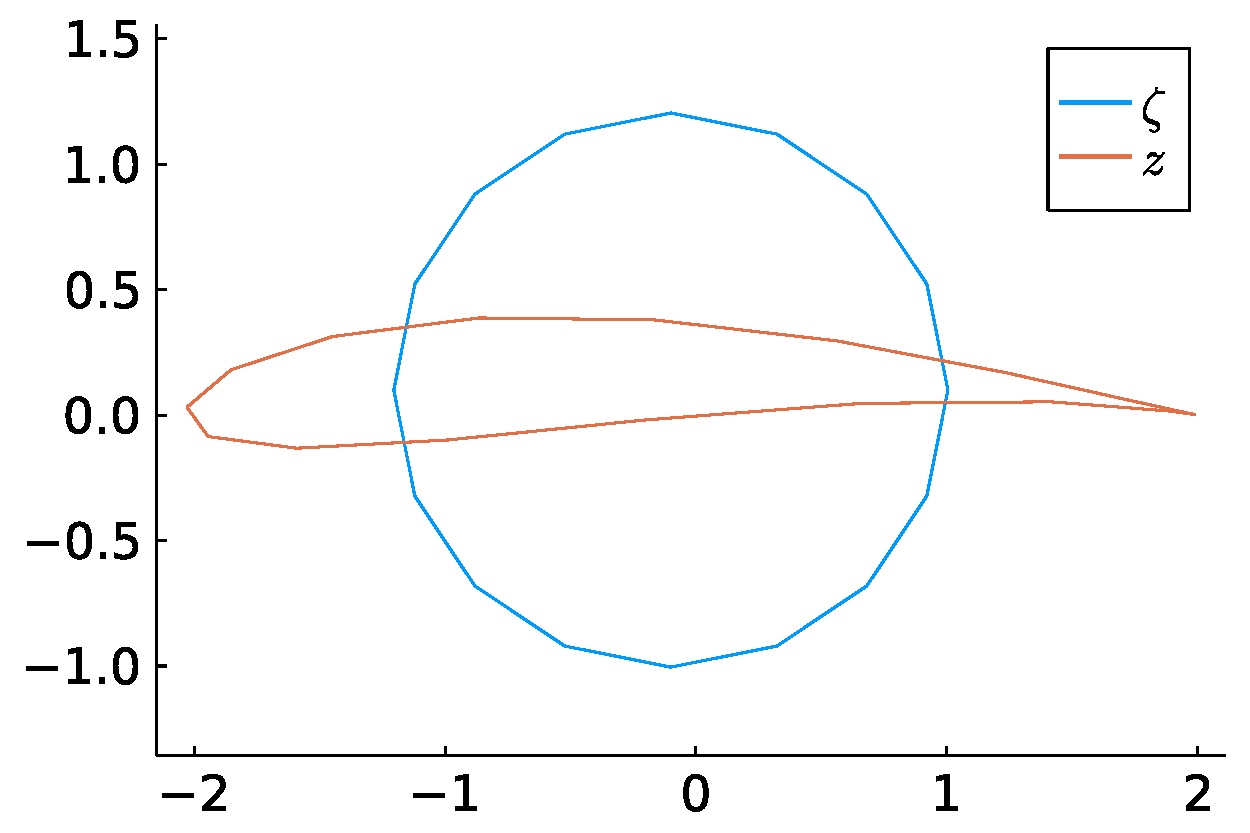
\includegraphics[width=8cm]{ZhukovskyWing.pdf}
    \caption{Zhukovsky変換の結果}
    \label{fig:zhukovsky}
\end{figure}

\section{結果と考察}
計算結果が解析解と定性的に一致しており, 正しく問題を解くことができたと考えられる.

\printbibliography[title=参考文献]
\end{document}